% 
% Annual Cognitive Science Conference
% Sample LaTeX Paper -- Proceedings Format
% 

% Original : Ashwin Ram (ashwin@cc.gatech.edu)       04/01/1994
% Modified : Johanna Moore (jmoore@cs.pitt.edu)      03/17/1995
% Modified : David Noelle (noelle@ucsd.edu)          03/15/1996
% Modified : Pat Langley (langley@cs.stanford.edu)   01/26/1997
% Latex2e corrections by Ramin Charles Nakisa        01/28/1997 
% Modified : Tina Eliassi-Rad (eliassi@cs.wisc.edu)  01/31/1998
% Modified : Trisha Yannuzzi (trisha@ircs.upenn.edu) 12/28/1999 (in process)
% Modified : Mary Ellen Foster (M.E.Foster@ed.ac.uk) 12/11/2000
% Modified : Ken Forbus                              01/23/2004
% Modified : Eli M. Silk (esilk@pitt.edu)            05/24/2005
% Modified : Niels Taatgen (taatgen@cmu.edu)         10/24/2006
% Modified : David Noelle (dnoelle@ucmerced.edu)     11/19/2014

%% Change "letterpaper" in the following line to "a4paper" if you must.

\documentclass[10pt,letterpaper]{article}
\usepackage{authblk}
\usepackage{cogsci}
\usepackage{pslatex}
\usepackage{apacite}
\usepackage{physics}
\usepackage{graphicx}
\usepackage{amssymb}
\usepackage{amsmath}
\usepackage{caption}
\usepackage{subcaption}
\usepackage{booktabs}
\hyphenpenalty=1000
\usepackage{xcolor}
\definecolor{Blue}{RGB}{50,50,200}
\definecolor{Green}{RGB}{50,200,50}
\definecolor{Red}{RGB}{200,50,50}
\newcommand{\hh}[1]{\textcolor{Blue}{@hh: #1}}
\newcommand{\cl}[1]{\textcolor{Green}{@cl: #1}}

\DeclareMathOperator*{\argmin}{arg\,min} % thin space, limits underneath in displays
\DeclareMathOperator*{\argmax}{arg\,max} % thin space, limits underneath in displays

\title{Evaluating machine comprehension of sketch meaning at different levels of abstraction}
 
%%% comment out authorship stuff for now

% \author[1]{\bf Kushin Mukherjee}
% \author[2]{\bf Holly Huey}
% \author[2]{\bf Xuanchen Lu}
% \author[3]{\bf Yael Vinker}
% \author[2]{\bf Rio Aguina-Kang}
% \author[2]{\bf Judith E. Fan}

% \affil[1]{University of Wisconsin-Madison, Madison, WI, United States}
% \affil[2]{University of California, San Diego, CA, United States}
% \affil[3]{Tel-Aviv University, Tel-Aviv, Israel}
% \author{\bf Anonymous CogSci Submission}
\begin{document}
% \makeatletter
% \let\@oldmaketitle\@maketitle% Store \@maketitle
% \renewcommand{\@maketitle}{\@oldmaketitle% 

% 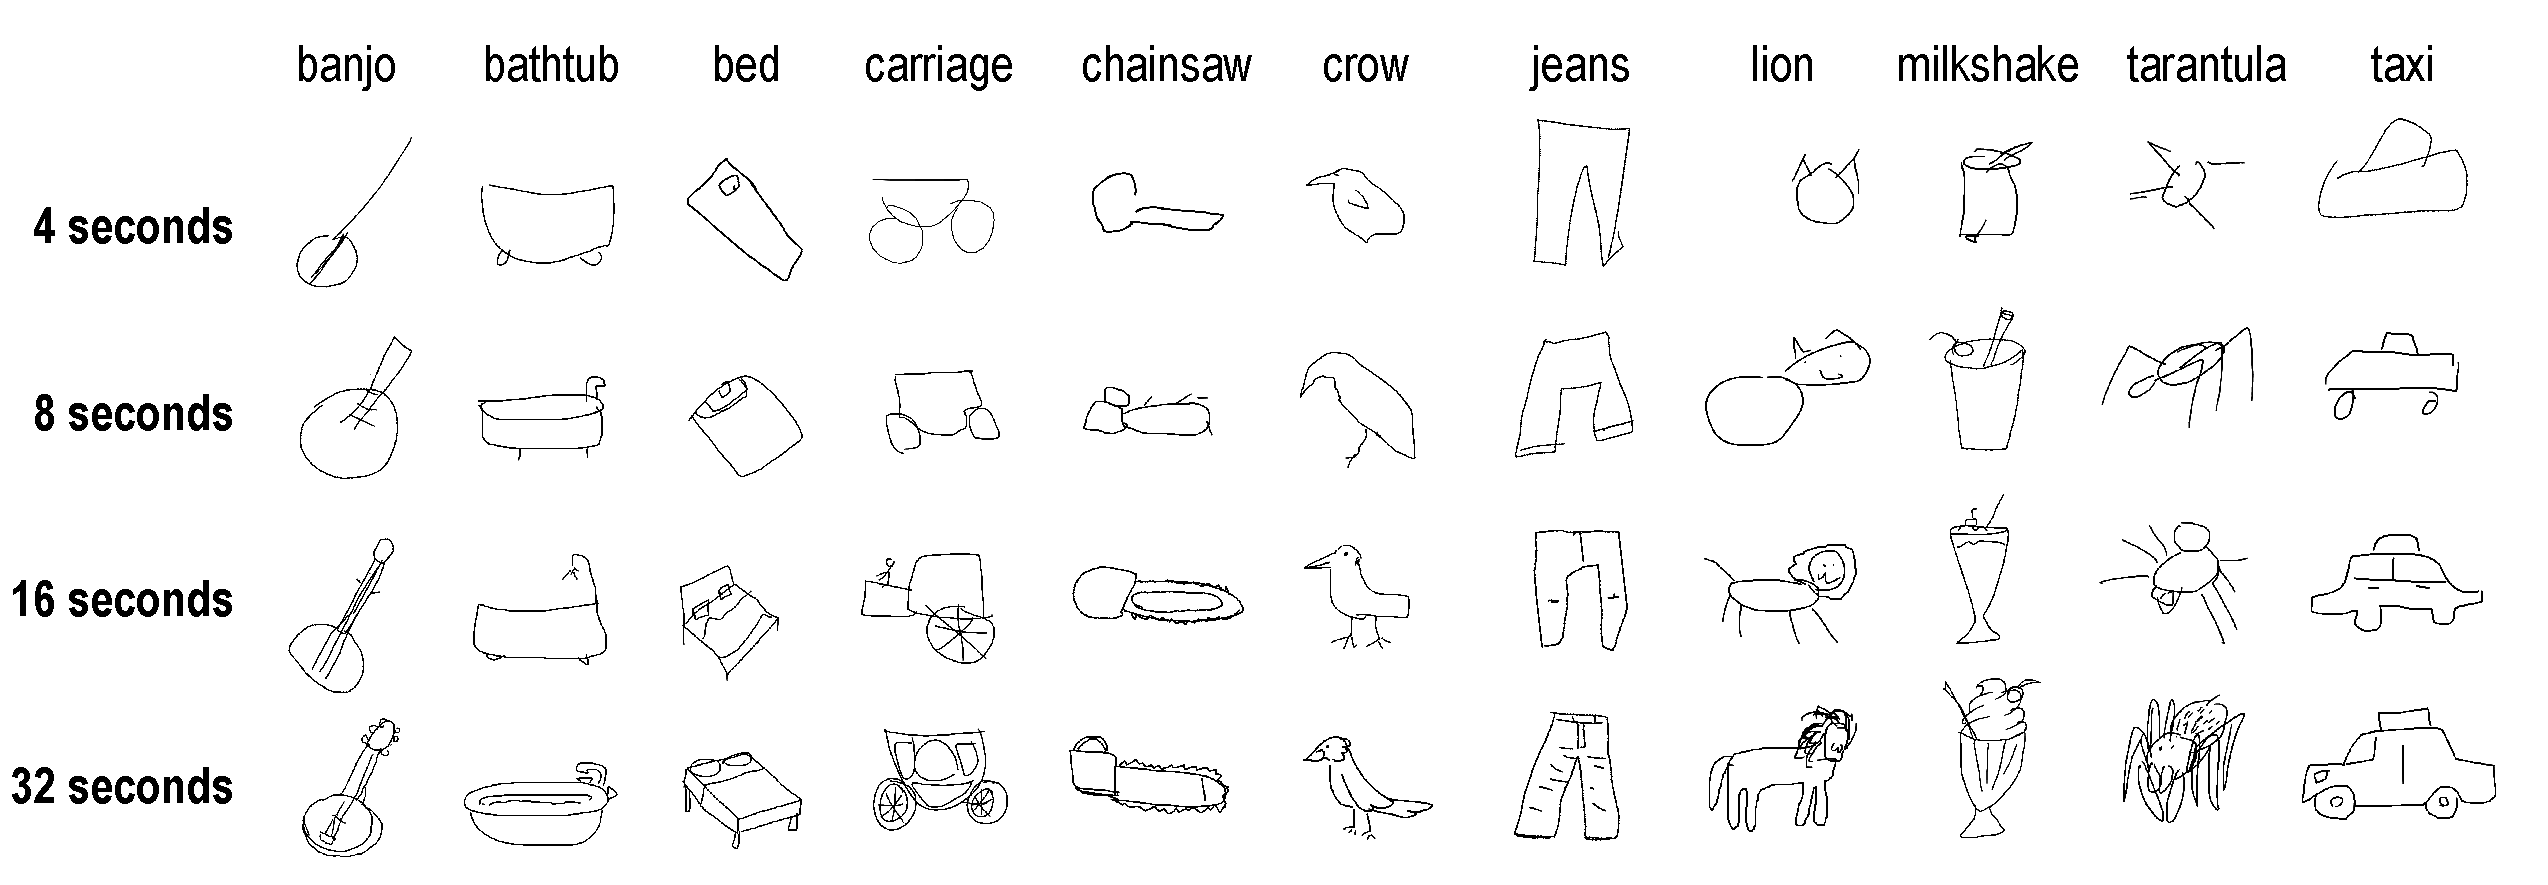
\includegraphics[width=.92\linewidth]{figures/thingsdraw_gallery_alpha.pdf}
% \captionsetup{width=0.92\textwidth}
%  \captionof{figure}{\footnotesize{Example sketches of objects from the THINGS128 dataset produced under different time limits.}}\

% }
% \makeatother
\maketitle
\begin{abstract}

People can understand images that vary in visual abstraction---from detailed illustrations to schematic icons. 
To what degree are current vision algorithms sensitive to such variation when encoding their meaning? 
We first obtained $>80K$ human-generated sketches produced under different time limits (4s, 8s, 16s, 32s; $N$=5,563 participants) and AI-generated sketches \cite{vinker2022clipasso} produced under different ink limits (8, 16, 32 strokes)  of 2,048 real-world objects spanning 128 categories from the THINGS dataset \cite{hebart2019things}.
We then evaluated how 13 state-of-the-art vision algorithms varying in architecture and training represented the meaning of these sketches, both at the category and exemplar levels, and without additional training.
We found that these models were generally sensitive to variation in visual abstraction, although some models were substantially more sensitive than others.
Together, these findings suggest promising avenues for building better models of human visual abstraction. 

\textbf{Keywords:} 
concepts; drawing; perception; computer vision; benchmark
\end{abstract}


\section{Introduction}

Humans can use pictures to convey what they perceive and know at varying levels of abstraction---from detailed illustrations to simple sketches.
Indeed, the ability to abstract away from the particulars of any given experience to highlight the most important elements is inherent in the act of creating any effective visualization \cite{viola2017pondering, chen2020foundations,mccloud1998understanding, mi2009abstraction, nan2011conjoining}.
Line drawings present an especially important case study in the capacity for visual abstraction, as demonstrated by the Spanish artist Pablo Picasso in his work, \textit{The Bull} (1945), which contains 11 lithographs of bulls, each successively more abstract than the last (Fig.~\ref{fig:bulls}).
Despite striking variation in their degree of fidelity to the real world, understanding what even the most abstract of these images represent feels effortless for most human viewers.

Such variation is not only manifest in works of art, but is pervasive across many domains of human activity. 
% , line drawings present an important case study in visual abstraction given their versatility and ubiquity in human culture.
Not only do most cultures produce drawings \cite{gombrich1995story}, the ability to produce line drawings that capture key aspects of the real world also emerges early in development \cite{karmiloff1990constraints, dillon2021rooms, long2021parallel}, and the visual properties of these drawings have been linked to children's developing conceptual knowledge \cite{tversky1989parts,huey2022developmental}. 
Additionally, failures to produce and understand pictures of objects at different levels of abstraction is associated with semantic dementia \cite{bozeat2003duck, rogers2007object}, suggesting links between a robust capacity for visual abstraction and the functional organization of semantic knowledge in the brain. 
What are the core visual computations that support this ability to grasp the meaning of pictures across so many different levels of visual abstraction? 

% of the world—objects, scenes, and events—at varying levels of abstraction. 
% Humans have the ability to visually communicate their knowledge of the world—objects, scenes, and events—at varying levels of abstraction. 
% could both depict scenes with incredible detail and attention towards preserving the likeness to the real world, as well as depict concepts like ``dog'' with only a single stroke by omitting much of the information that would help the sketch share a visual resemblance to a real dog. 
% The relevance and necessity to abstract visually across many different levels arises across many instances of visual communication.
% In certain contexts, a faithful and detailed depiction might be what is required, such as when an architect conveys detailed schematics to an engineer \cite{suwa1997architects} or when a zoologist creates scientific illustrations of a new animal species \cite{baigrie1996picturing}. 
% However in other contexts, such as when there exists established social conventions or when resources are limited (e.g., time), simpler depictions can be used to efficiently denote objects \cite{fan2020pragmatic, garrod2007foundations, hawkins2021visual}. 
% Amongst these cases, one tool for visualization that might showcase the greatest variability in visual abstraction while being widely pervasive are line drawings \cite{sayim2011line}.

\begin{figure}[t]
    \centering
    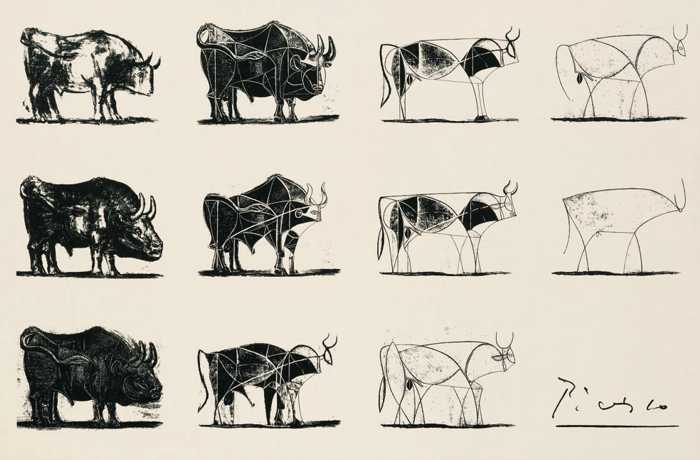
\includegraphics[width= 0.8\linewidth]{figures/picasso_bulls.jpg}
    \caption{Pablo Picasso. \textit{The Bull}, 1945.}
    \label{fig:bulls}
    \vspace{-2em}
\end{figure}
% both kinds of depictions can be understood and recognized by those who view them. 

% This notion that knowledge can be flexibly expressed and understood at many such levels of abstraction, while raised in prior work  \cite{viola2017pondering, chen2020foundations,mccloud1998understanding}, has evaded a generalized formal account. 
% As a consequence, it has remained unclear to what degree modern vision algorithms can support varied representations of the same underlying concept spanning multiple degrees of abstraction.

% While many might agree that knowledge can be flexibly expressed and comprehended at such different levels of abstraction, a formal account of visual abstraction has remained largely absent in the .
% For example, in the domain of sketching, a sketcher can choose to produce a highly-detailed realistic drawing or a simplified stylized drawing. 
% From an observer's perspective, the former might be evocative of a specific flower, such as a rose, the latter might convey the general concept of 'flower'. 

% Thus, drawings are ubiquitous in culture and development, a window into learned semantics, and exhibit variation in perceived abstractness.
% These properties make drawings of real-world objects a uniquely well-suited vehicle for understanding visual abstraction and developing common protocols for measurement of this construct across humans and machines mirroring similar efforts in cognitive science and AI \cite{bear2021physion}.

The past several years have seen remarkable progress in uncovering the mechanisms by which the human visual system achieves a robust understanding of the visual world \cite{yamins2014performance, kriegeskorte2015deep, zhuang2021unsupervised, konkle2022self}. 
These mechanistic models now often take the form of trainable neural networks combining several architectural motifs inspired by the primate ventral visual stream 
% including its hierarchical organization and local circuit properties 
\cite{gross1972visual,goodale1992separate,malach2002topography,hung2005fast}. %--- though not in all cases \cite{dosovitskiy2020image}.
These advances have also recently been applied to the problem of sketch understanding, revealing both the value of these approaches to learning general-purpose perceptual representations to model human visual abstraction \cite{fan2018common, yu2017sketch, kubilius2016deep}, as well as persistent challenges in achieving the capacity for robust understanding of visual inputs that vary in their degree of visual abstraction \cite{baker2018abstract, singer2022photos, fan2020pragmatic}.

% \begin{figure*}[ht!!]
\begin{figure}[ht!]
    \centering
    \includegraphics[width= .85 \linewidth]{figures/VAB_task_vertical.pdf}
    \vspace{-1em}
    \caption{Human sketch production task and machine generated sketches
    % (A) Examples of photo exemplars from the THINGS dataset.
    % % The current study included a total of 2,048 visual objects spanning 128 visual concepts from the THINGS dataset \cite{hebart2019things} 
    % (B) Human participants generated sketches under 4 conditions: 4s, 8s, 16s, and 32s time restrictions. \textit{CLIPasso} 
    % % \cite{vinker2022clipasso} 
    % generated sketches of the same photos under 3 conditions: 8-stroke, 16-stroke, and 32-stroke restrictions.
    % Both humans and an AI system, \textit{CLIPasso} \cite{vinker2022clipasso}, generated sketches of concrete visual objects under different production constraints. Human participants were asked to create a sketch of the abstract concept represented in a photograph under a certain time limit (i.e., 4s, 8s, 16s, and 32s). \textit{CLIPasso} created a sketch based on the photograph using a certain number of strokes (i.e., 8 strokes, 16 strokes, 32 strokes).
    }
    \vspace{-2em}
    \label{fig:trial}
\end{figure}

Despite these great strides in the development of high-performing vision models, it remains unclear to what degree the \textit{specific} models that have been proposed so far achieve human-like understanding of such a broad range of visual inputs, from natural images to human-generated drawings and symbols.
Evaluating this question has been especially challenging given that, while there are several widely used benchmark sketch datasets \cite{eitz2012sketch, jongejan2017quick, sangkloy2016sketchy}, none of them systematically vary the abstraction level of the sketches they contain. 

In this paper, we take two major steps towards closing this gap: 
(1) to develop a large dataset containing human ($N$=5,563 participants) and AI-generated sketches that vary in their degree of abstraction, for a representatively wide variety of visual object concepts; 
and (2) to systematically evaluate how well various state-of-the-art vision models, varying in their architectures and training methods, represent semantic information about these sketches, including information about the target object at the category and exemplar levels, without additional training. 
We build on a growing body of research leveraging a global image dataset generated by the THINGS initiative \cite{hebart2019things} by sampling 2,048 real-world objects spanning 128 concepts as referents for the drawings in our dataset.
Here, specifically, we leverage the drawings to investigate which axes of variation among vision models might be most salient for human-like understanding of drawings.
We propose metrics for measuring sensitivity to visual abstractionm, which constitute a meaningful new dimension along which all future vision model can be evaluated along.

Taken together, our work aims to contribute an informative benchmark of human and machine generated sketches spanning varying multiple levels of abstraction. 
By publicly releasing these datasets as well as our proposed metrics for investigating sketch understanding, these data generate opportunities for future research avenues towards building better computational models of human visual abstraction.
% \textit{first,} we collected a large number of human-generated sketches produced under different time limits (4s, 8s, 16s, 32s; $N$=5,563 participants) and AI-generated sketches \cite{vinker2022clipasso} produced under different ink limits (8, 16, 32 strokes) of 2,048 real-world objects spanning 128 categories from the THINGS dataset \cite{hebart2019things}. \textit{Second,} we conducted a systematic evaluation of how well several state-of-the-art vision algorithms, varying in their architecture and training, represent the meaning of these sketches, without additional training.
% Taken together, our study aims to provide a useful benchmark dataset and framework for probing sketch understanding in machines, and point to promising avenues for building better computational models of human visual abstraction in future work.

% A critical requirement for such efforts is a dataset depicting a sufficiently diverse set of objects at varying levels of abstraction. Using a time-restricted drawing paradigm, we present such a dataset of human-produced drawings depicting 2048 exemplars of 128 unique concepts. We also leverage recent advances in machine sketch-generation \cite{vinker2022clipasso} to create machine-produced drawings at varying levels of abstraction. Next, we evaluate a suite of modern vision algorithms which vary in their architectures, training paradigms, and training datasets, in their sensitivity to variations in abstraction. While we find many dimensions of variance across latent neural representations in their ability to capture variations in abstractness, we show that convolutional neural networks and models trained on semi-supervised learning methods are among the most sensitive to these variations.

% This serves as an important first step towards the systematic study of visual abstraction in both humans and machines.

% This body of work from diverse areas of cognitive science lends support to the notion that


% \subsection{Computational models of vision}
% Deep learning models, including convolutional neural networks (see \citeNP{li2021survey} for a review) and vision transformers \cite{dosovitskiy2020image}, are often considered the best contemporary models of human visual perception \cite{kriegeskorte2015deep,kubilius2019brain,lindsay2021deep} even in the domain of drawings \cite{fan2018common}. But how sensitive are these algorithms to semantic abstraction of the kinds described earlier? Here, we first collect a dataset of human and machine sketches .... spanning different levels of visual abstraction. Next, we evaluate representations extracted from a suite of vision models at various stages of processing (early, intermediate, and late) to measure their ability to represent visual concepts at different levels of abstraction using novel formalizations of visual abstraction.

% \section{Sketching at varying levels of abstraction}

\section{Method}
% The current paper has two key aims: 
% (1) to develop a large dataset containing human and AI-generated sketches that vary in their degree of abstraction, for a wide variety of visual object concepts; 
% and (2) to evaluate how well various state-of-the-art vision models represent semantic information about these sketches, including information about the target object at the category and exemplar levels, without additional training. 
Our first goal was to generate two parallel large-scale drawing datasets spanning varying levels of abstraction: one produced by humans under varying time limits (4s, 8s, 16s, and 32s), and the other by automatic machine generation varying in the number of strokes per drawing (8, 16, and 32 strokes), using CLIPasso \cite{vinker2022clipasso}.  

% In order to generate human drawings that spanned a variety of abstractions, we adapted a time-restricted drawing task used in work by \citeauthor{berger2013style} (2013) and asked people to produce drawings of objects in 4, 8, 16, and 32 seconds.
% Here we hypothesized that under time constraints, people would produce drawings that are not only less detailed but also more evocative of the general concept they were asked to draw, relative to a specific instance of that concept.


\subsubsection{Stimuli}
% THINGS database
To generate a diverse large-scale stimuli set of object concepts, we systematically sampled 128 concepts from the database of the THINGS initiative, a global database of 1,854 object concepts (e.g., ``chair'', ``elephant'', ``airplane'') and naturalistic object images aimed at developing a multi-varied cognitive neuroscience and behavioral metrics on a shared set of objects \cite{hebart2019things}. 
Building on prior work by \citeauthor{yang2021visual} (2021) investigating visual abstraction across different contexts, we selected concepts based on similar parameters spanning four main axes of variation: familiarity, artificiality, animacy, and size. 
Within each object concept, we randomly sampled 16 object images. 
Our final stimuli set included 2,048 object images that were used as visual referents for our human and machine sketching tasks.

\subsection{Human Sketch Production Task} 
\subsubsection{Participants} 
5,563 participants (2,870 male; $M_{age}$ = 36.7 years) were recruited from Prolific to produce a series of sketches on a web-based drawing platform. 
Data collection stopped when 10 sketches had been generated for each of the 2,048 object images.
We excluded 104 data sessions from participants who experienced technical difficulties.
Participants provided informed consent in accordance with our institution’s IRB.

\subsubsection{Procedure}
Participants were randomly assigned to one of four conditions, each varying in the amount of time that they were permitted to use to generate their drawings: 4, 8, 16, or 32 seconds. 
During each drawing trial, participants were presented with a label cue of an object concept, a corresponding object image (500px x 500px) as an example of the concept, and a drawing canvas (500px x 500px) and were instructed to draw the concept that they were presented with (Fig. \ref{fig:trial}). 
Beside the canvas, participants were given a countdown timer indicating how many seconds they had left to produce their drawing. 
To ensure that participants were prepared to draw given the short duration of each condition, a reminder about the drawing duration was interleaved between drawing trials that also provided participants the opportunity to take a short break and to indicate when they were ready to start the next trial. 
A trial ended when the timer ran out or if the participant pressed the ``Continue'' button if they finished their sketch with time remaining, although they were instructed to try to use as much time as they needed to accurately represent the prompted concept.
They were also permitted to undo their most recent stroke or completely clear their canvas if needed. 

Each participant produced 16 drawings of different object concepts.
Prior to drawing trials, participants were provided specific instructions that they were to draw the general concept of presented objects and that, although the provided object image was an example of the concept, they should not include details that were specific to the object in the image. 
Additionally, they were instructed not to include any background context (e.g., grass in a drawing of a ``horse''), arrows, or text.
Participants also completed a practice trial before the test drawing trials to familiarize themselves to the drawing platform.


\subsection{Machine Generated Sketches}
In addition to human drawings, we leveraged Vinker et al.'s \citeyear{vinker2022clipasso} CLIPasso model to generate sketches of our 2,048 images at multiple levels of abstraction.
CLIPasso is a recently developed method for object sketching, in which the parameters of a predefined set of curves (strokes) are optimized to depict a given image of an object, guided by a pre-trained CLIP \cite{radford2021learning} model.
Different levels of abstraction are achieved by varying the number of strokes used. 
For each image in the 2,048 set, we generated sketches at three levels of abstraction using 8, 16, and 32 strokes (see Figure \ref{fig:trial} for example) as an approximately parallel manipulation of the time-restriction paradigm we leveraged to collect our human drawing dataset. 
While our preliminary analyses made use of 3 levels of abstraction due to computing limitations, in the future we will aim to have a more varied and granular set abstraction levels to augment our set of human sketches.

% We also leveraged recent advances in sketch-generation algorithms, namely the CLIPasso model \cite{vinker2022clipasso}, to generate sketches at different levels of abstraction. 
% We sampled a single exemplar photo for each concept and generated sketches at 3 levels of abstraction for those photos. Since CLIPasso varies abstraction by varying the total number of strokes the model uses to create the sketch we had the model produce sketches with 8, 16, and 32 strokes (Figure \ref{fig:clipasso_ex}. 

% \begin{figure}
%     \centering
%     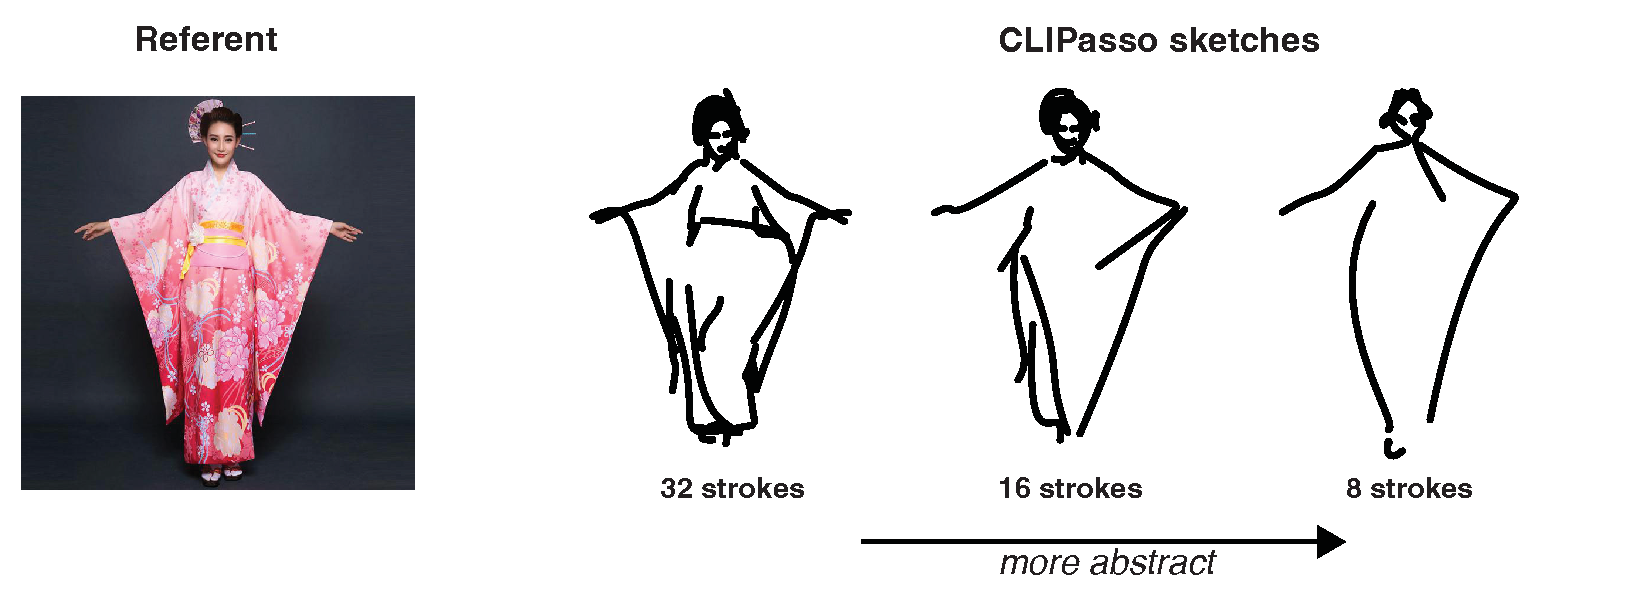
\includegraphics[width=.5\textwidth]{figures/clipasso.pdf}
%     \caption{Machine generated sketches of a photograph at low (32 strokes), medium (16 strokes), and high (8 strokes) levels of abstraction}
%     \label{fig:clipasso_ex}
% \end{figure}

% \begin{figure*}
%     \centering
%     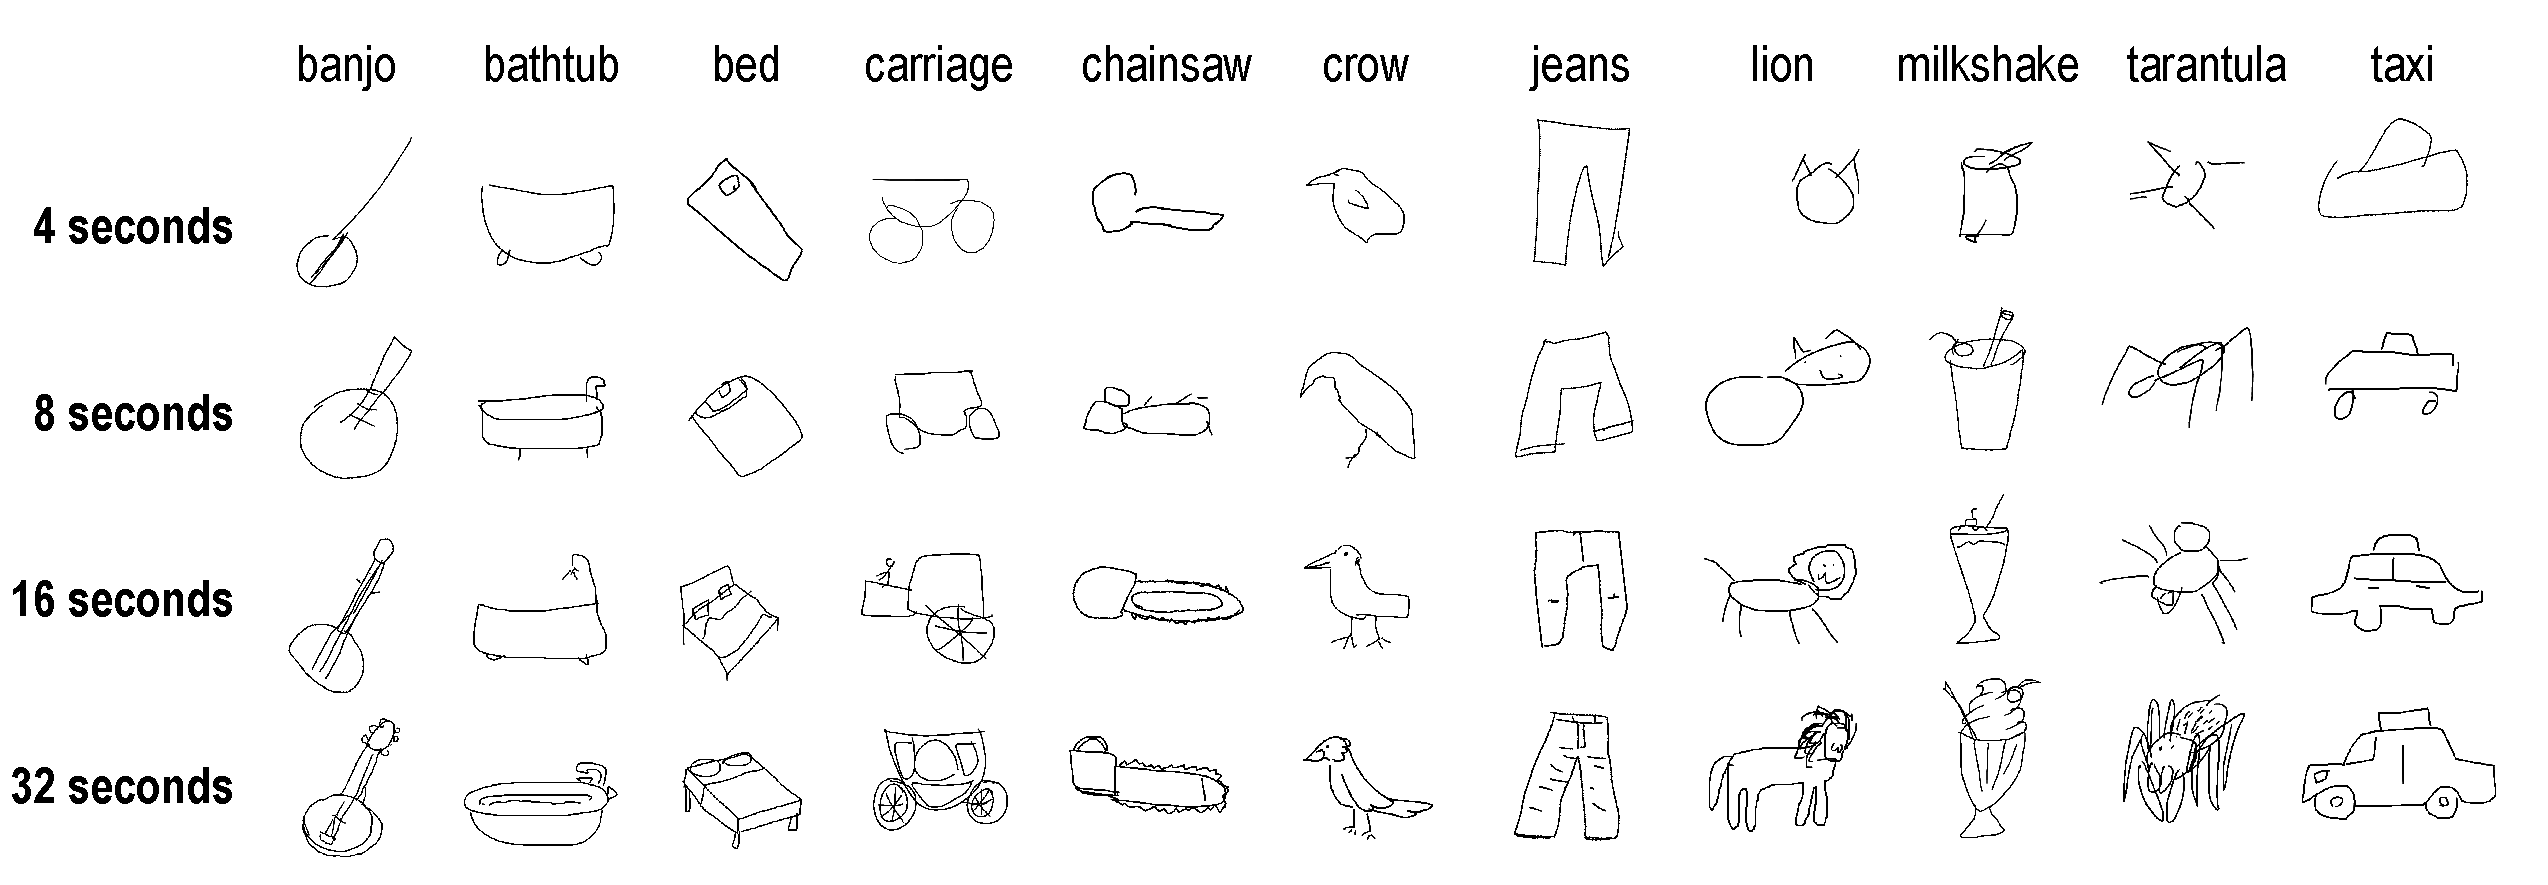
\includegraphics[width= 1\linewidth]{figures/thingsdraw_gallery_alpha.pdf}
%     \caption{Example sketches of objects from the THINGS128 dataset produced under different time limits.}
%     \label{fig:gallery}
% \end{figure*}

% \subsubsection{Results}
% \hh{We collected over 84,000 unique drawings of the THINGS128 dataset. 
% We first tested if there were any meaningful differences between drawings of the same concept across the different timing conditions.
% To accomplish this, we measured the number of unique strokes in a drawing as a metric of the amount of detail included in each drawing and fit a mixed-effects linear regression model with random intercepts for concept type predicting number of strokes as a function of time allotted per drawing showed a significant effect of time.
% We found that drawings produced under the 4s limit contained the least number of average strokes, whereas those produced under the 32s limit contained the most number of average strokes ($\beta=.029$, $t=58.54$, $p<.001$, see Table \ref{tab:strokes} for all four conditions). 
% These results confirm that the time-restriction manipulation elicited meaningful differences in detail across drawing conditions.} 
% % The amount of detailed included in each drawing, measured using the number of unique strokes in a drawing, did increase with increased allowed drawing time with the 4s condition having the fewest strokes and the 32s condition having the most strokes on average. Refer to table \ref{tab:strokes} for information on all 4 conditions.
% % A mixed-effects linear regression model with random intercepts for concept type predicting number of strokes as a function of time allotted per drawing showed a significant effect of time ($\beta=.029$, $t=58.54$, $p<.001$). Thus, our time-restriction manipulation did indeed lead to drawings that varied in level of detail. 
% In order to answer our questions about visual abstraction, we define two complementary metrics to measure the amount of abstraction in a sketch based on its latent representations. 

% \begin{table}[h!]
%     \centering
%     \begin{tabular}{c|l l}
%         Drawing time & $M_{strokes}$ & $SD_{strokes}$\\
%          \toprule
%         4 seconds & 1.61 & 1.49\\
%         8 seconds & 3.49 & 2.43\\
%         16 seconds & 6.39 & 4.27\\
%         32 seconds & 9.90 & 7.11\\
%         \bottomrule 
%     \end{tabular}
%     \caption{Differences in number of strokes used per drawing condition. Longer drawing times resulted in more detailed drawings, but also a greater variance in amount of detail included }
%     \label{tab:strokes}
% \end{table}


\section{Formalizing abstraction in vision models}
\begin{figure}[ht!]
    \centering
    \includegraphics[width=0.8\linewidth]{figures/VAB_schematic2.pdf}
     \vspace{-1em}
    \caption{Calculating metrics: (1) cosine similarities between sketch embeddings and each photo are computed to generate category and exemplar-level similarity distributions; (2) classification accuracy is measured by whether the correct category/exemplar is among the 10 most similar items.
    % Procedure for computing visual abstraction metrics for a given sketch. Cosine similarities between embeddings for the sketch and each of the 2,048 photographs are computed to generate distributions of category and exemplar level similarities. Classification accuracy is measured by whether the correct exemplar/category is among the 10 most similar items.
    }
    \vspace{-1em}
    \label{fig:_}
    \vspace{-0.5em}
\end{figure}

What properties of state-of-the-art vision models hinder or facilitate comprehension of visual concepts at varying levels of abstraction? 
To make progress towards answering this question, we first curated a set of vision models with varied architectural commitments and training procedures. 
Next, we formalized a set of metrics for relating latent representations extracted from deep layers of the model to our questions regarding sensitivity to semantic information at different levels of abstraction.

% Beyond object recognition and scene segmentation, robust vision algorithms should be more sensitive to an image's abstractness relative to less human-like algorithms. Further, what properties of a vision model might hinder or facilitate visual abstraction comprehension? In order to answer this question, we curated a set of vision models with a varied architectural commitments and training procedures. We then describe methods for relating latent representations extracted from early, intermediate, and late layers of the models, of sketches to those of the THINGS128 dataset in order to define a formal set of metrics for visual abstraction.

% ... We would like to investigate 1) how models differ in their sensitivities to the level of abstraction and 2) how this ability varies in the early, intermediate, and late representations of vision models. To investigate the   se problems, we first proposed two metrics, specificity and genericity, that quantitatively measure the model sensitivity to variation in abstraction. We then evaluated a variety of vision models with their early/intermediate/late representations and [other analysis].

\subsubsection{Models} 
We evaluated 13 models spanning multiple architectures (Convolutional Networks (convnets), transformers, and Multi-layer Perceptrons (mlps)) and training paradigms (supervised learning, self-supervised learning, and semi-supervised learning) to investigate the effects of these factors on models' sensitivity to visual abstraction. 
The models include 3 ImageNet-supervised ConvNets \cite{deng2009imagenet}, 3 ImageNet-supervised transformers, 4 self-supervised vision models, CLIP, and 2 semi-supervised models (see Table \ref{tab:models}). 
We performed all downstream computations on latent features extracted from the deepest non-mlp layers of these models. This amounted to extracting activation patterns at either the model's final convolution or attention layer.


% \begin{table}[htp]
% \centering
% % \vspace{-4mm}
% \resizebox{0.5\textwidth}{!}{%
% \begin{tabular}{l|l|l|l}
% Methods  & Architecture & Training Paradigm & Dataset\\ 
% \hline
% VGG-19~\cite{simonyan2014very} & VGG-19 & supervised & ImageNet\\ 
% Inception-V3~\cite{szegedy2016rethinking} & Inception-V3 & supervised & ImageNet\\
% ResNet-50~\cite{he2016deep} &  ResNet-50  & supervised & ImageNet \\
% ViT-B~\cite{dosovitskiy2020image}  & ViT-B & supervised & ImageNet \\
% Swin-B\cite{liu2021swin} & Swin-B & supervised & ImageNet \\ 
% MLPMixer-B~\cite{tolstikhin2021mlp} & MLPMixer-B & supervised & ImageNet \\ 
% MoCo-v2~\cite{chen2020improved} & ResNet-50 & self-supervised & ImageNet \\ 
% MoCo-v3~\cite{chen2021empirical} & ViT-B & self-supervised & ImageNet \\ 
% DINO~\cite{caron2021emerging} & ViT-B & self-supervised & ImageNet \\ 
% MAE~\cite{he2022masked} & ViT-B & self-supervised & ImageNet \\ 
% CLIP~\cite{radford2021learning} & ViT-B & self-supervised & WebImageText \\ 
% Noisy Student~\cite{xie2020self} & EfficientNet-b4 & semi-supervised & ImageNet + JFT \\
% SWSL~\cite{yalniz2019billion} &  ResNet-50  & semi-supervised & ImageNet + 1B-Targeted \\
% \bottomrule 
% \end{tabular}%
% }
% %\vspace{1mm}
% \caption{The list of models that we evaluated. We show the network architecture, training paradigm, and training dataset of each model.}
% % \vspace{-5mm}
% \label{tab:models}
% \end{table}



\begin{table}[htp!]
\centering
\vspace{-0.5em}
\resizebox{0.5\textwidth}{!}{%
\begin{tabular}{l|l|l}
Models  & Architecture & Training Paradigm\\ 
\hline
\textbf{VGG-19}~\cite{simonyan2014very} & VGG-19 & supervised \\ 
\textbf{Inception-V3}~\cite{szegedy2016rethinking} & Inception-V3 & supervised \\
\textbf{ResNet-50}~\cite{he2016deep} &  ResNet-50  & supervised  \\
\textbf{ViT-B}~\cite{dosovitskiy2020image}  & ViT-B & supervised\\
\textbf{Swin-B}\cite{liu2021swin} & Swin-B & supervised\\
\textbf{MLPMixer-B}~\cite{tolstikhin2021mlp} & MLPMixer-B & supervised\\
\textbf{MoCo-v2}~\cite{chen2020improved} & ResNet-50 & self-supervised \\
\textbf{MoCo-v3}~\cite{chen2021empirical} & ViT-B & self-supervised\\
\textbf{DINO}~\cite{caron2021emerging} & ViT-B & self-supervised\\
\textbf{MAE}~\cite{he2022masked} & ViT-B & self-supervised \\
\textbf{CLIP}~\cite{radford2021learning} & ViT-B & self-supervised\\
\textbf{Noisy Student}~\cite{xie2020self} & EfficientNet-b4 & semi-supervised\\
\textbf{SWSL}~\cite{yalniz2019billion} &  ResNet-50  & semi-supervised \\
\bottomrule 
\end{tabular}%
}
\vspace{-0.5em}
\caption{Models evaluated and their network architecture backbone and training paradigm.}
\vspace{-1em}
\label{tab:models}
\end{table}
\subsubsection{Visual abstraction metrics} 

A hallmark of human visual knowledge is the ability to categorize an object at different levels of granularity from broad categories to specific instances \cite{mervis1981categorization}. In our human sketch production task, participants were prompted to draw concepts with a photographic referent to ground the visual concept. 
Under resource constraints, one might imagine that a sketcher would dedicate strokes and ink towards communicating features that would be generally evocative of the concept, while with greater resources they might include visual information borrowed from the specific referent photograph.
Under less drawing time, we predicted sketches to be more abstract and to evoke general \textit{category} level information.
On the other hand, with more drawing time, we predicted sketches to be more detailed and concrete and to evoke information about a specific \textit{exemplar}.
We define two classification-based metrics to capture these ideas:
% \hh{To measure the level of abstraction contained within each generated sketch, we use two main metrics of visual abstraction:} 

% \cl{To measure the sensitivity of models to the level of abstraction contained within each drawing, we use two metrics to evaluate how well the models match the drawing to its corresponding exemplar or category:} 
% We considered two main desiderata for a measure of a sketch's level of abstraction and grounded them in concrete metrics. 
\begin{itemize}

    % % \item \textbf{Specificity} Secondly, for an abstract sketch, the measure should not provide strong evidence for \textit{any} specific exemplar of \textit{any} concept either.\\
    % \item \textbf{Specificity} \hh{As drawings increase in abstraction, they lose their specificity to a particular exemplar of a concept (e.g., the least abstract cow drawn by Picasso might be identified as a specific real-world cow, whereas a more abstract cow meres evokes the general concept of a cow). Here, we predicted that more abstract drawings would be less similar to the example photo that was displayed during the drawing task.}
    \item \textbf{Exemplar-level classification accuracy} This evaluates the ability of model embeddings to correctly assign a given sketch to the corresponding exemplar photograph that was either used as a referent the human sketching task or used as input to CLIPasso for machine sketch generation.
    % An abstract sketch should not be particularly evocative of any particular exemplar. Here, a sketch should not be highly similar to the referent photo that was displayed during the drawing task.
    % Thus, the greater the degree of abstraction in a sketch, the lesser its specificity.    
    % \item \textbf{Genericity} \hh{Conversely, as drawings increase in abstraction, they provide \textit{stronger} evidence for the correct concept depicted in a drawing relative to evidence for a particular instance of that concept. Here, we operationalize this metric such that more abstraction corresponds to lower genericity score.}
    \item \textbf{Category-level classification accuracy} This evaluates the ability of model embeddings to correctly assign each sketch to its corresponding object category. 
    
    % \cl{I suggest we collapse this itemmized motivation section, because the two metrics are too similar.}
    
    % If a sketch is abstract, the measure should provide \textit{stronger} evidence for the correct concept depicted in a drawing relative to evidence for a particular instance of that concept. Here, for consistency with specificity, we will operationalize the metric such that more abstraction corresponds to lower genericity score.
    % \item \textbf{Genericity} Firstly, if a sketch is abstract, the measure should provide strong evidence for the correct concept (relative to other concepts) but not any specific exemplar of that concept.

\end{itemize}

\noindent To mathematically formalize these two metrics, we denote the set of sketches as $S$, photo exemplars as $E$, and categories as $C$. 
Additionally, we denote the extracted feature embeddings of the $2048$ photo exemplars given a vision model as $F_{E} \in \mathbb{R}^{2048\times channel}$ and denote the extracted embedding of sketches from the human sketch production set as $F_{S} \in \mathbb{R}^{num\_sketches\times channel}$.
% Given a vision model and a selected early/intermediate/late layer, we extracted the feature embeddings of the $2048$ photo exemplars, denoted $F_{E} \in \mathbb{R}^{2048\times channel}$. Similarly, we extracted the embedding of sketches from the human sketch production set as $F_{S} \in \mathbb{R}^{89419\times channel}$.
We computed the embedding of each of the 128 categories as the mean embedding of the corresponding 16 photo exemplars, denoted $F_{C} \in \mathbb{R}^{128 \times channel}$.

We used cosine similarity to calculate the similarity between any given sketch's embeddings $s\in S$ and the 2048 photo exemplars $E$, resulting in a similarity matrix $\mathbb{R}^{1 \times 2048}$. Then we consider the exemplar with the maximum value in the similarity matrix as the exemplar-level classification result, denoted $Y_{E}^{(s)}$.
%= \{y_E_1^{(s)}, ..., y_E_k^{(s)}\}$. 
%that we normalize with the softmax function, giving a probability distribution $P_{E}^{(s)}$ that represents the probability that the sketch corresponds to each of the 2048 photo exemplars. 
% Similarly, we computed the probability distribution $P_{concept}^{(i)}$ that consists of the probability that the sketch corresponds to each concept. 
Similarly, we computed the similarity matrix $\mathbb{R}^{1 \times 128}$ between a given sketch $s$ and categories $C$. The category-level classification result are then $Y_{C}^{(s)}$.
%= \{y_C_1^{(s)}, ..., y_C_k^{(s)}\}$.
Formally, we therefore have:
\begin{equation}\label{eq:p exemplar}
    Y_{E}^{(s)} = \argmax_{e\in E} (Similarity(F_{S}^{(s)}, F_{E})),
\end{equation}
\vspace{-0.5em}
\begin{equation}\label{eq:p category}
    Y_{C}^{(s)} = \argmax_{c\in C} (Similarity(F_{S}^{(s)}, F_{C})),
\end{equation}
where $Similarity$ is the cosine similarity.

In practice, for a more stable statistics, instead of a simple $\argmax$, we retrieve the 10 best exemplars/categories corresponding to the sketch $s$ as the top-10 classification results $Y^{(s)} = \{y_1^{(s)}, ..., y_k^{(s)}\}$. The top-10 classification accuracy, as a result, measures the percentage in which the correct label $y_{true}^{(s)}$ is among the top 10 results predicted.

% With the probability distributions ready,
% We now detail the formulation of the two metrics.


% \textbf{Specificity score.} 
% % As mentioned in the two desiderata, a highly abstract sketch should not strongly correspond to its photo exemplar. Therefore, 
% The specificity metric $L_{Specificity}$ measures how strongly a sketch matches its corresponding photo exemplar, treating all other exemplars as distractors. We formulated the problem as selecting the correct exemplar out of the 2048 photos. Given the sketch $s$ and its correct exemplar $e_{true}^{(s)}\in E$, the metric is computed as the reciprocal of the cross entropy between the one-hot target distribution $\delta^{(s)}$ and the probability distribution $P_{E}^{(s)}$,

% \begin{equation}\label{eq:specificity}
%     L_{Specificity}^{(s)} =-\frac{1}{\sum_{e\in E}{\delta^{(s)}(e) \log{[P_{E}^{(s)}(e)}]}},
% \end{equation}

% where 
% \begin{equation}\label{eq:one hot}
%     \delta^{(s)}(e) :=
%     \begin{cases}
% 1 &\text{if } e = e_{true}^{(s)}, \\
% 0 &\text{if } e \neq e_{true}^{(s)}.
% \end{cases}
% \end{equation}



% % To compute the specificity of a sketch, we measure the KL-divergence between the idealized and empirical instance level distributions. The larger this term the less abstract a sketch is.

% % $$S(s) = D_{KL}(p(s)_{instance},\delta_{instance}(s))$$
% % \textbf{Results}



% \textbf{Genericity.} 
% The genericity metric $L_{Genericity}$ measures how strongly a sketch corresponds to a concept without evoking any particular exemplar within the concept category.
% This can be formalized as a ratio between the likelihood of assigning the drawing to the photo that was the referent during the human production experiment and the likelihood of assigning the drawing to the correct category. The smaller this number is, the less likely one is to correctly assign the drawing to the exemplar relative to correctly assigning it to the concept. This would be a drawing that evokes a concept more generally without evoking a particular exemplar.

% Given the sketch $s$, its correct exemplar $e_{true}^{(s)}\in E$ and its correct concept $c_{true}^{(s)} \in C$, the metric is computed as the ratio between the cross-entropy between the one-hot target distribution $\delta_{C}^{(s)}$ and probability distribution $P_{C}^_{(s)}$ and the cross-entropy between the one-hot target distribution $\delta_{E}^{(s)}$ and probability distribution $P_{E}^{(s)}$,

% \begin{equation}\label{eq:genericity}
%     L_{Genericity}^{(s)} =-\frac{\sum_{e\in E}{\delta_{E}^{(s)}(e) \log{[P_{E}^{(s)}(e)}]}}{\sum_{c\in C}{\delta_{C}^{(s)}(c)  \log{[P_{C}^{(s)}(c)}]}},
% \end{equation}

% where 
% \begin{equation}\label{eq:one hot}
%     \delta_{E}^{(s)}(e) :=
%     \begin{cases}
% 1 &\text{if } e = e_{true}^{(s)}, \\
% 0 &\text{if } e \neq e_{true}^{(s)},
% \end{cases}
% \end{equation}
% and
% \begin{equation}\label{eq:one hot}
%     \delta_{C}^{(s)}(c) :=
%     \begin{cases}
% 1 &\text{if } c = c_{true}^{(s)}, \\
% 0 &\text{if } c \neq c_{true}^{(s)}.
% \end{cases}
% \end{equation}



% \begin{figure*}[ht!!]
%     \centering
%     \includegraphics[width=.95\textwidth]{figures/VAB_all_mod.pdf}
%     \caption{Average genericity and specificity scores for sketches made in each timing condition based on latent features extracted from each model in our model suite at early, intermediate, and late stages of processing. }
%     \label{fig:all_models}
% \end{figure*}


\section{Results}


\subsubsection{Shorter drawing times produce sketches with less strokes}
Our final drawing dataset contained over 84,000 unique drawings. 
To test the effect of our manipulation, we first measured the number of unique strokes in a drawing as a metric of the amount of detail.
Then, we fit a mixed-effects linear regression model with random intercepts for category predicting number of strokes as a function of time allotted per drawing showed a significant effect of time.
We found that drawings produced under the 4s limit contained the least number of average strokes, whereas those produced under the 32s limit contained the most number of average strokes ($\beta=.029$, $t=58.54$, $p<.001$, see Table \ref{tab:strokes} for all conditions). 
These results confirm that the time-restriction manipulation elicited meaningful differences in detail across drawing conditions.
\vspace{-.8em}
\begin{table}[ht!]
\centering
    \begin{tabular}{c|l l}
        Drawing time & $M_{strokes}$ & $SD_{strokes}$\\
         \toprule
        4 seconds & 1.61 & 1.49\\
        \vspace{-1mm}
        8 seconds & 3.49 & 2.43\\
        16 seconds & 6.39 & 4.27\\
        32 seconds & 9.90 & 7.11\\
        \bottomrule 
    \end{tabular}
    \vspace{-0.5em}
    \caption{Number of strokes used per drawing condition. 
    % Longer drawing times resulted in more detailed drawings, but also a greater variance in amount of detail included 
    }
    \label{tab:strokes}
    \vspace{-2em}
\end{table}

% \subsubsection{Models are sensitive to differences in human and machine drawings made under different constraints}
\subsubsection{Models detect meaningful differences in sketches made under different constraints}
% The time-restricted drawing task and stroke-number manipulation in CLIPasso resulted in sketches that varied in the overall level of detail. 
How successfully are extant vision algorithms, trained to be sensitive to semantic information, able to support varied sketch representations of the same concept made under different resource constraints? 

To answer this question we investigated whether models' ability to classify a sketch at the category or exemplar level varied as a function of drawing time for humans and number of strokes for machine drawings. 
We fit a series of mixed effects linear regression models predicting exemplar and category classification accuracy from drawing duration (for humans) and number of strokes (for CLIPasso) with a by-category random intercept and by-model random intercept and random slope for time duration/number of strokes. 
For humans, we found a significant effect of drawing time on exemplar level classification ($\beta = 8.49\times10^{-04}$, $p < .05$) and category level classification ($\beta = 2.68\times10^{-03}$, $p < .05$) with longer drawing times being associated with higher accuracy. 
We found converging evidence from machine generated sketches with greater number of strokes being associated with higher classification accuracy at the exemplar ($\beta = 0.003$, $p < .01$) and category level ($\beta=.004$, $p < .05$).
Thus, current vision algorithms are indeed sensitive to visual differences in drawings made by both humans and machines under different resource constraints.

\subsubsection{Model training affects sensitivity to semantic information in drawings}
% \subsubsection{Model training techniques affect sensitivity to semantic information in drawings although more for human drawings than machine drawings.}

What are the effects of a model's architecture and training objective on a its ability to decode semantic information in a drawing at different levels of abstraction? 
To understand the contributions of these two sources of variation, we tested the effects of architecture and training technique on models' abilities to classify sketches at the exemplar and category level (Figure \ref{fig:train_arch}).
We represented architectures and training techniques using dummy codes, with convnets and supervised training as the reference levels.
For both human and machine drawings, we compared mixed-effects linear regression models predicting classification accuracy from drawing time (number of strokes for machines) and architecture type to models with only drawing time or number of strokes as a predictor. 
We specified the same random effects structure as earlier and fit models for both exemplar and category level classification.
For human sketches, we did not find a significant contribution of architecture at the exemplar level ($\chi^2(2) = 4.44$ $p = .11$) but did find support for architecture sensitivity at the category level ($\chi^2(2) = 9.68$, $p < .05$).
There were no meaningful differences of different architectures in classification of machine-generated sketches at either the category ($\chi^2(2) = .30$, $p=.90$) or exemplar level ($\chi^2(2) = 2.76$, $p=.25$).

To assess the role of training technique on models' abilities to represent human and machine sketches at different levels of abstraction, we compared mixed-effects linear regression models predicting top-10 classification accuracy from drawing time (number of strokes for machines) and training method to models with only drawing time as a predictor. 
We found support for the notion that models trained using different techniques were sensitive to differences in semantic information conveyed by human drawings at both the exemplar ($\chi^2(2) = 14.90$, $p < .001$) and category level ($\chi^2(2) = 10.89$, $p<.005$) to different degrees.
This sensitivity was not observed for machine drawings, where model comparisons were not significant at either the exemplar ($\chi^2(2) = .74$, $p=.70$) or category level ($\chi^2(2) = 1.68$, $p=.43$).

Taken together, our results show that while vision algorithms are able to support varied representations for drawings made under different constraints, the role of architecture (convnet vs. mlp vs. transformer) is limited relative to the choice of training technique (supervised vs. unsupervised vs. semi-supervised). Notably, the absence of an effect of architecture and training on decodability of semantic information from machine generated sketches emphasises the importance of human behavioral data to distinguish between models on their ability to support visual abstractions.

\begin{figure}[ht!]
    \centering
    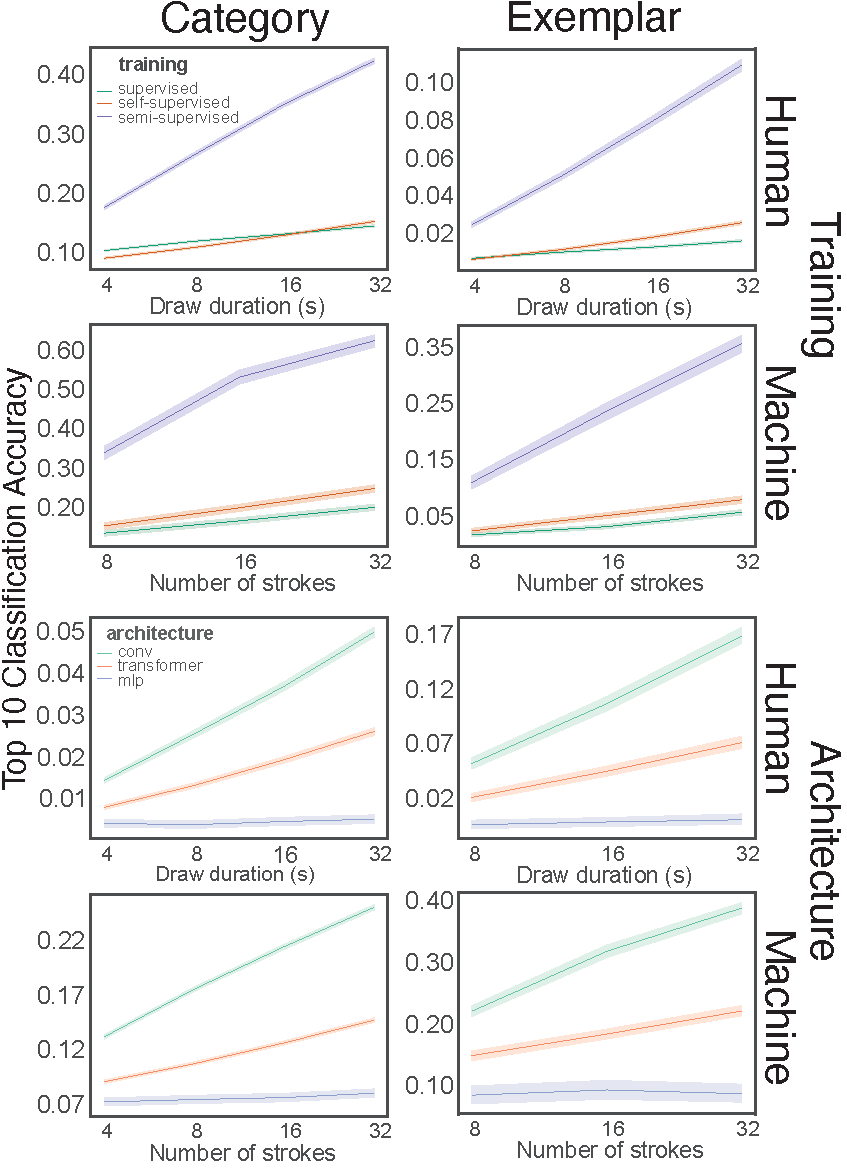
\includegraphics[width=.48\textwidth]{figures/VAB_train_arch.pdf}
    \vspace{-2em}
    \caption{Effect of training algorithm (top) and architecture (bottom) on visual abstraction metrics.}
    \label{fig:train_arch}
    \vspace{-2em}
\end{figure}

\subsubsection{Model properties moderate sensitivity to semantic information under different constraints}
% \subsubsection{Sensitivity to semantic information in both human and machine drawings at different constraint levels is moderated by properties of models}
\begin{figure*}
    \centering
    \includegraphics[width=.95\textwidth]
    {figures/VAB_all_mods.pdf}
    \vspace{-0.5em}
    \caption{(A) Sketch classification performance by models. (B) Model-model consistency in classification performance. Darker colors indicate greater consistency.}
    \label{fig:all_mods}
    \vspace{-1.5em}
\end{figure*}

While we have shown that vision models \textit{on average} are sensitive to both exemplar level and category level semantic information to varying degrees depending on the level of constraint imposed (time or strokes), is this sensitivity to constraint-level moderated by, on a coarse level, the architecture and training of the model, and on a granular level, the model itself? (See Figure \ref{fig:all_models} for a birds-eye view of every model benchmarked and their performance at different levels of abstraction).

To answer these questions, we fit mixed effects linear regression models predicting accuracy from draw duration (humans) and number of strokes (machines) and their interactions with dummy-coded versions of (1) model name, (2) architecture, and (3) training. 
We specified random intercepts per drawing category.
We compared these models to nested models that did not contain the interaction terms to assess the moderating influence of these factors on the effect of constraint.

For both human sketches, the interaction of model $\times$ constraint was significant at both the exemplar ($\chi^2(12) = 2017.4$, $p <.001$) and category level ($\chi^2(12) = 2238.60$,$p <.001$).
This was also true for machine generated sketches at both the exemplar ($\chi^2(12) = 1237.10$, $p < .001$) and category level ($\chi^2(12) = 598.68$, $ p <. 001$). 
This shows that different models process the semantic information at different abstraction levels in different ways.

Collapsing across models sharing the same architecture, we found no significant interaction of architecture $\times$ constraint in predicting top-10 accuracy for human sketches at the exemplar ($\chi^2(2) = 1.8$, $p = .55$) and category level ($\chi^2(2) = 1.96$, $p = .37$). 
A similar result was observed for machine sketches at the exemplar ($\chi^2(2) = 2.78$, $p = .25$) and category level ($\chi^2(2) = 5.82$, $p = .05$).
This adds support to the notion that, at least among the models considered here, architecture is not a significant contributor to any observed difference in model performance at the categorical or exemplar level. 

By contrast, we found a significant effect of the interaction between model training $\times$ constraint for human sketches at the exemplar($\chi^2(2) = 9.89$, $p < .01$) and category level($\chi^2(2) = 11.23$, $p < .005$).  This result was replicated for machine sketches where model comparisons showed a significant effect of training $\times$ constraint on exemplar level ($\chi^2(2) = 13.87$, $p < .001$) and category level accuracy ($\chi^2(2) = 12.71$, $p < .005$).

Overall, these results cohere with results from the previous section in highlighting the importance of training methods on models' sensitivity to visual abstraction.

\subsubsection{Shared model architectures have consistent sensitivity to semantic information}
% \subsubsection{Models sharing the same architecture are consistent in their representations of sketches}

While architecture isn't generally predictive of a models' sensitivity to drawings made under different constraints, are models belonging to a architecture class coherent in their sensitivity to semantic information in sketches? That is, do different models sharing common architectures have similar patterns of performance on exemplar and category level classification?

To test this hypothesis, we constructed similarity matrices of classification performance by computing the pairwise Pearson correlations of exemplar and category classification performance between each model at each constraint level (see Figure \ref{fig:all_mods}(B)).
For both the category and exemplar level performance similarity matrices, we computed the ratio of the average \textit{within-architecture} similarity to average \textit{between-architecture similarity}. We generated a null-distribution for this ratio by permuting the row assignments for the similarity matrix generating dataset 10000 times. We found that the probability of observing the true ratio or higher was $.<001$ for both the category level and exemplar level similarity matrices, which supports the notion that models that share an architecture are more consistent in their performance relative to models that have different architectures. Performance on machine generated sketches similarly showed greater within-model consistency relative to between-model consistency ($p<.001$) for both exemplar level and category information.

Thus, while there are limited differences in the performance \textit{between} model architectures measured by how well their representations of sketches can be decoded to yield semantic information at varying levels (exemplar vs categorical), the performances \textit{within} an architecture class also hang together consistently.

% \subsubsection{Current models share similar sketch representations of visual abstraction}
\subsubsection{Models have consistent sensitivity to semantics across abstraction levels}
% \subsubsection{Models are consistent in their representations of sketches made under different constraints}

While there is consistency within model architectures in the degree to which they are sensitive to semantic information, is there a meaningful effect of constraint level (time or number of strokes) on performance across all models? 
 Are models' understanding of sketches made under lighter constraints—more drawing time, greater number of strokes—more varied relative to sketches made under tighter constraints? If different models are sensitive to different visual features, which might arise with more detailed drawings, one might expect to see a negative correlation between constraint level and performance consistency.

To test this hypothesis, we once again constructed model-model performance similarity matrices at both the exemplar and category level. 
We computed the average similarity within each constraint condition (4 for human drawings, 3 for machine drawings) and estimated the slope of the relationship between these 2 factors. 
To test the statistical significance of the slope we permuted the matrix-generating dataset 10000 times and constructed a null-distribution of similarity-by-constraint slopes. Under this distribution the observed true slopes were not significant at either the exemplar ($p_{human} = .86$,$ p_{machine}  = .81$) or category level ($p_{human}  = .82$, $p_{machine} = .99$). 
Thus, current vision models are consistent in their sensitivities to semantic information across different abstraction conditions




% The full picture of every model being benchmarked along with specificity and genericity metrics derived at early, intermediate, and late stages of processing can be seen in figure \ref{fig:all_models}. Certain general trends can be observed, such as a greater processing of abstraction across the time-restricted conditions in deeper layers of most models captured by a significant positive interaction between model depth $\times$ timing condition (genericity: $\beta_{model\_depth \times time} = $1.69, $t =$21.74, $p<$.05; specificity:$\beta_{model\_depth \times time} = $3.24, $t =$43.05, $p<$.05 ). This aligns with the notion that deeper stages of processing in deep neural networks represent their input in a more categorical manner abstracted away from the specific image statistics of the input \cite{yamins2014performance,khaligh2014deep,rajalingham2018large}. 

% While we established that our time-restriction manipulation resulted in less detailed drawings, often a signature of abstraction, for shorter drawing times are these drawings really more abstract? 
% To evaluate the hypothesis that shorter drawing times lead to more abstract representations we first investigated whether drawings made under greater time pressure led to more abstract representations in vision models as measured by our abstraction metrics.

% A linear mixed-effects model with random intercepts for the referent image concept showed a significant effect of drawing time, with drawings made with more time showing greater specificity ( $\beta =$ 1.79e-05, $t=$ 28, $p<$.05) and also greater genericity ( $\beta =$ 4.05e-05, $t=$ 65.55, $p<$.05).
% Thus, as resources such as time become scarce, the more abstract people's depictions of concepts become.

% While convolutional neural networks have garnered sustained interest as some of the best performing models of human vision \cite{yamins2014performance,cadieu2014deep,kriegeskorte2015deep,kietzmann2019recurrence}, there have yet to be systematic investigations into the ability of convnets and other vision algorithms to represent the same concept at multiple levels of abstraction on a large-scale dataset such as ours.
% Thus we ask, do models that have inductive biases similar to those of human biological vision have an advantage in discerning abstractness in drawings?
% We investigated this by asking how model architecture might influence models' ability to represent increasingly sparse sketches across our different drawing time conditions.
% We grouped the model architectures broadly into 3 classes — convolution-based models (convnets), transformer-based models, and models relying primarily on multi-layer perceptrons \cite{tolstikhin2021mlp}— and represented abstraction metrics generated from each class of model using dummy codes with convnets as the reference class. We used these predictors in conjunction with drawing time and their interactions to fit a mixed-effects linear regression model with random intercepts per concept predicting both abstractness metrics.
% We found that the effect of time-restriction on abstraction was weaker in mlp and transformer architectures relative to convolutional models (figure \ref{fig:gen_spec} (left column)).
% This was supported by a significant effect of model class $\times$ timing condition on both the specificity (
% $\beta_{mlp \times time}= $ -5.81e-06, $t =$ -24.23, $p<$.05; $\beta_{transformer \times time}= $ -3.19e-06, $t =$ -24.88, $p<$.05) and genericity metrics (
% $\beta_{mlp \times time}= $ -3.50e-05, $t =$ -35.12, $p<$.05; $\beta_{transformer \times time}= $-1.92e-05 , $t =$ -24.88, $p<$.05). While transformers continue to drive much progress in natural language process and vision \cite{chen2021visformer}, our results point to the continued relevance of convnets in modeling aspects of human visual cognition.


% Along with variations in architecture, a variety of optimization regimes or training techniques have arisen in recent years that have improved model performance on standard benchmarks such as ImageNet classification \cite{deng2009imagenet}. Do these innovations in training protocols bear on our question of visual abstraction? 
% To answer this question, we first grouped techniques into 3 classes — supervised learning methods, unsupervised learning methods, and semi-supervised methods (see table \ref{tab:models} for a full list). Once again we dummy coded these conditions, treating supervised learning as the reference class and fit a linear-mixed effects model in the same manner as we did for architecture, replacing those terms with terms for training techniques. The interaction of training technique $\times$ timing condition for both semi-supervised and unsupervised was positive in both the specificity ($\beta_{supervised \times time}= $ 1.17e-06, $t =$ 8.77, $p<$.05; $\beta_{semi-supervised \times time}= $ 9.03e-06, $t =$ 49.90, $p<$.05) and genericity model $\beta_{supervised \times time}= $ 6.76e-06, $t =$12.13, $p<$.05; $\beta_{semi-supervised \times time}= $ 5.54e-05 , $t =$ 73.70, $p<$.05).
% While both metrics point towards semi-supervised and self-supervised training methods better capturing the effect of time-restriction on abstraction, as can be seen in figure \ref{fig:gen_spec} (right column), the magnitude of this effect is greatly pronounced for representations derived from models trained using semi-supervised techniques.





% \begin{figure}
%     \centering
%     \includegraphics[width=.5\textwidth]{figures/VAB_all_mods.pdf}
%     \caption{Model-model consistency in classification performance at the category and exemplar level for both human and machine generated sketches. Darker colors indicate greater consistency.}
%     \label{fig:cormat}
% \end{figure}

\vspace{-1em}
\section{Discussion}

Humans' ability to connect highly abstract visual tokens to meanings provides the basis for understanding not only pictorial representations \cite{hawkins2021visual, garrod2007foundations}, but also for the development of symbolic writing and numeral systems over time \cite{schmandt2010writing, chrisomalis2020reckonings}. 
In this paper, we introduce a new large-scale drawing dataset based on 2,048 objects spanning diverse 128 concept categories that has systematic variability in the level of visual abstraction drawings are depicted in.
Our dataset combines both human-made drawings and machine-made drawings made under varying resource constraints leading to diversity in abstraction level.
We also provide initial benchmarking of a representative set of vision models spanning architectures and training techniques. We broadly find evidence that current models are sensitive to the differences semantic information conveyed in sketches across levels of abstraction though models don't agree on the structure of information present.
While the contributions of architecture towards this sensitivity is limited, different models belonging to the same architecture do cohere together.
The effect of training, specifically self-supervised learning methods, leads to the greatest sensitivity to visual abstraction.

We view our work as complementary to efforts seeking to understand the contributions of the different components that make up current AI vision models towards their performance \cite{hermann2020shapes, nguyen2020wide,schott2021visual,chen2021intriguing}. Here, we consider an aspect of visual cognition as fundamental as it is evasive to formalize — visual abstraction — and evaluate models on their sensitivity to this construct. Future work will seek to benchmark a wider variety of models including those inspired by cognitive neuroscience \cite{chen2022unsupervised, zhuang2021unsupervised,kubilius2019brain} and will seek to build more robust metrics of abstraction beyond those tied to classification-based accuracy.

% \section{Acknowledgments}

% The authors would like to thank members of the Cognitive Tools Lab at UC San Diego for their comments and support. This work was supported by NSF CAREER Award #2047191 to J.E.F.


\bibliographystyle{apacite}

\setlength{\bibleftmargin}{.125in}
\setlength{\bibindent}{-\bibleftmargin}

\bibliography{references}


\end{document}
